\section{研究背景}
随着社会的数据隐私保护意识的提升和相关法律法规的出台,许多隐私保护机器学习方法被提出。
%
拆分学习~\cite{vepakomma2018split,poirot2019split}作为纵向联邦学习~\cite{liu2024vertical}的一种主要方法,有着效率较高、实现简单的优势,因此获得了工业界和学术界的广泛关注~\cite{palanisamy2021spliteasy,koda2020split_mmwave,fagbohungbe2022split_edge_image,roth2022split_unet}。
%


\begin{figure}[htbp]
    \centering
    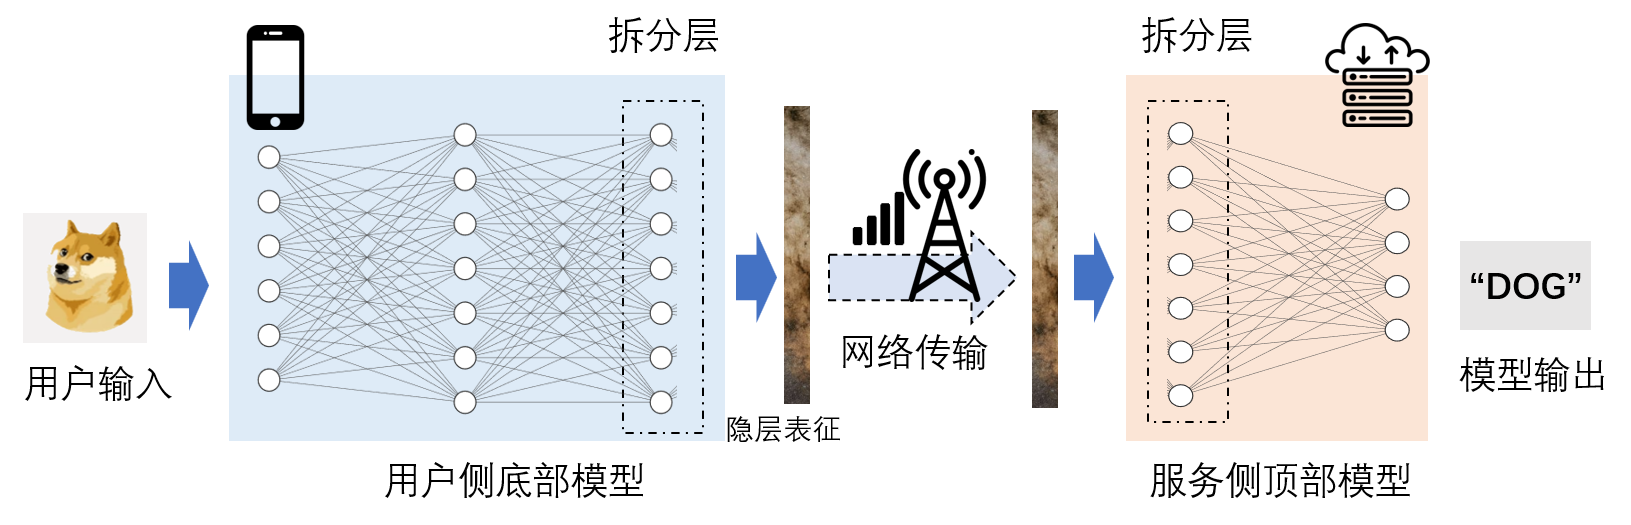
\includegraphics[width=\linewidth]{Z_Resources/随机topk_两方拆分学习示意图.png}
    \caption{两方拆分学习推断示意图}
    \label{fig:randomized_topk-split_example}
\end{figure}

拆分学习的思想是把模型拆分成多个部分分发给各个参与方,各方以交换中间结果的方式进行模型训练和推断,从而实现一定程度上的隐私保护。
%
\autoref{fig:randomized_topk-split_example}显示了一个典型的两方拆分学习的推断场景,我们假设用户具有输入数据,而服务器拥有一个分类模型。
%
进行拆分学习的推断时,用户拥有底部模型,而服务器拥有顶部模型。用户将输入输入底部模型获得隐层表征后,通过网络传输给服务器,然后将其输入顶部模型,从而得到最终的模型预测值。
%
在此过程中,用户只暴露了输入数据的隐层表征,因此其原始输入获得了一定的保护;而服务器只暴露了底部模型而非完整模型,因此模型的隐私也在一定程度上得到了保护。
%
虽然拆分学习的效率相对于密码学方法很高,但是由于拆分学习训练过程中依然需要在每一轮传输隐层特征和梯度,考虑到许多深度学习模型的隐层空间较大,因此拆分学习在通讯效率上依然存在可以优化的空间。
%



本文主要关注类别数量多的深度学习模型场景。
%
分类模型往往可以拆分为特征抽取器和分类器两个部分,其中,特征抽取器的结构较为复杂,可以包含卷积层、长短期记忆层等;而分类器可能是一层简单的全连接层。
%
但是在类别数量众多的情况下,分类器往往包含了模型的大部分参数,如:
%
推荐系统模型~\cite{jannach2017gru4rec,kang2018sasrec}的最后一层可能包含了所有商品的嵌入向量(Embedding Vector);
%
人脸识别模型~\cite{parkhi2015deepface}的最后一层可能包含了所有用户的人脸对应的嵌入向量。
%
在这种情况下,若简单地将整个模型部署到用户侧,既会占用大量的用户侧存储空间,也会带来模型隐私泄露的风险。
%
因此,在这种情况下,就需要采用拆分学习的方式来提高效率,同时保护用户输入和模型参数的隐私。

当前关于纵向联邦学习通讯压缩的研究相对较少,仅有对基础压缩算法的收敛性分析~\cite{castiglia2022compressed_vfl}、拆分层嵌入自编码器~\cite{ayad202vfl}等,前者仅考虑了基本的压缩方法且只应用于训练阶段,而后者只针对拆分学习的一个特定场景。
%
关于提升横向联邦学习的通讯效率的工作则较多,包括了加快收敛速度~\cite{karimireddy2020scaffold,reddi2020fed_opt}、压缩每一轮传输的梯度值~\cite{wen2017terngrad,aji2017sparse,sattler2019sparse_binary}等。
%
前者并不适用于拆分学习,因此本文主要研究如何压缩拆分学习训练和推断过程中传递的中间结果或中间梯度信息。
%

